\documentclass[11pt,a4paper]{article}

% -----------------------------------------------------------------------------
% Packages
% -----------------------------------------------------------------------------
\usepackage[a4paper,left=33mm,right=33mm,top=30mm,bottom=32mm]{geometry}
\usepackage[utf8]{inputenc}
\IfFileExists{lmodern.sty}{\usepackage[T1]{fontenc}\usepackage{lmodern}}{}
\usepackage{microtype}
\usepackage{amsmath,amssymb,amsthm,mathtools}
\usepackage{graphicx}
\usepackage{booktabs}
\usepackage{tabularx}
\usepackage{array}
\usepackage{enumitem}
\usepackage{xcolor}
\usepackage{caption}
\usepackage{float}
\usepackage{placeins}
\usepackage{listings}
\usepackage[nottoc]{tocbibind}
\usepackage[round,authoryear]{natbib}
\usepackage[hidelinks]{hyperref}
\usepackage[nameinlink,capitalise,noabbrev]{cleveref}

\hypersetup{
  pdftitle={From Ideal Points to Robot Joints: Computational geometry and conformal geometric algebra},
  pdfauthor={Yana Osinchuk},
  pdfsubject={Seminar paper, Applied Mathematics, Hochschule Darmstadt},
  pdfkeywords={computational geometry, homogeneous coordinates, conformal geometric algebra, inverse kinematics}
}

% -----------------------------------------------------------------------------
% Layout
% -----------------------------------------------------------------------------
\setlength{\parindent}{0pt}
\setlength{\parskip}{0.45em}
\setlist{nosep,leftmargin=1.6em}
\emergencystretch=2em
\widowpenalty=10000
\clubpenalty=10000
\setcounter{tocdepth}{2}
\captionsetup{font=small,labelfont=bf,skip=6pt}
\captionsetup[table]{position=top}
\renewcommand{\arraystretch}{1.12}
\newcolumntype{Y}{>{\raggedright\arraybackslash}X}

% -----------------------------------------------------------------------------
% Theorem-like environments
% -----------------------------------------------------------------------------
\theoremstyle{plain}
\newtheorem{proposition}{Proposition}
\newtheorem{lemma}{Lemma}
\theoremstyle{definition}
\newtheorem{definition}{Definition}
\theoremstyle{remark}
\newtheorem{remark}{Remark}
\crefname{proposition}{Proposition}{Propositions}
\crefname{lemma}{Lemma}{Lemmas}
\crefname{definition}{Definition}{Definitions}
\crefname{remark}{Remark}{Remarks}

% -----------------------------------------------------------------------------
% Code listings
% -----------------------------------------------------------------------------
\definecolor{codegray}{gray}{0.96}
\definecolor{commentgreen}{HTML}{2A7F62}
\definecolor{keywordblue}{HTML}{1F4E9A}
\lstdefinelanguage{CLUScript}{
  morekeywords={if,else},
  morekeywords=[2]{VecN3,SphereN3,DrawLine,Slider,DefVarsN3,SetMode,SetLineWidth,sqrt,Color,einf,e2},
  sensitive=true,
  morecomment=[l]{//},
  morestring=[b]"
}
\lstset{
  basicstyle=\ttfamily\scriptsize,
  keywordstyle=\color{keywordblue}\bfseries,
  keywordstyle=[2]\color{keywordblue},
  commentstyle=\color{commentgreen}\itshape,
  stringstyle=\color{black},
  numbers=left,
  numberstyle=\tiny\color{gray},
  numbersep=6pt,
  frame=lines,
  framerule=0.4pt,
  backgroundcolor=\color{codegray},
  breaklines=true,
  breakatwhitespace=true,
  columns=fullflexible,
  keepspaces=true,
  showstringspaces=false,
  xleftmargin=1.5em,
  aboveskip=0.6em,
  belowskip=0.6em
}

% -----------------------------------------------------------------------------
% Notation
% -----------------------------------------------------------------------------
\newcommand{\R}{\mathbb{R}}
\newcommand{\PP}{\mathbb{P}}
\newcommand{\GA}{\mathcal{G}_{4,1}}
\newcommand{\einf}{e_{\infty}}
\newcommand{\ezero}{e_{0}}
\newcommand{\T}{\mathsf{T}}
\newcommand{\norm}[1]{\left\lVert#1\right\rVert}
\newcommand{\abs}[1]{\left\lvert#1\right\rvert}
\newcommand{\bis}{\operatorname{bis}}
\newcommand{\conv}{\operatorname{conv}}
\newcommand{\proj}{\operatorname{proj}}
\newcommand{\Sph}{\mathcal{S}}
\DeclareMathOperator*{\argmax}{arg\,max}
\DeclareMathOperator*{\argmin}{arg\,min}

% Date of submission (edit here)
\newcommand{\SubmissionDate}{September 23, 2026}

% Numbers produced by code/generate_figures.py
\input{generated/results.tex}

\begin{document}

% =============================================================================
% Title page
% =============================================================================
\begin{titlepage}
  \hypersetup{pageanchor=false}
  \centering
  \hspace*{\fill}\includegraphics[width=0.5\textwidth]{figures/logo_hda.png}\par
  \vspace{34mm}
  {\bfseries Seminar paper in the field of Mathematics and Natural Sciences\\
   Bachelor's program in Applied Mathematics\par}
  \vspace{24mm}
  {\LARGE\bfseries From Ideal Points to Robot Joints\\[3pt]
   Computational geometry and\\[1pt] conformal geometric algebra\par}
  \vspace{22mm}
  {\large Yana Osinchuk\par}
  \vspace{9mm}
  {\large \SubmissionDate\par}
\end{titlepage}

% =============================================================================
% Front matter
% =============================================================================
\pagenumbering{roman}
\setcounter{page}{1}

\section*{Declaration}
\addcontentsline{toc}{section}{Declaration}

I affirm that I have independently authored this seminar paper and have not
used sources or aids other than those explicitly mentioned. Any directly quoted
or paraphrased passages from other works are appropriately acknowledged.

The Python programs that serve as part of the source material
(\cref{sec:source}) were developed jointly with a fellow student in the
practical part of the course. Generative AI tools were used as an aid for
language editing and for reviewing the program code; all derivations,
programs, and numerical results were checked by me.

\vspace{22mm}
\begin{tabular}{@{}p{0.42\textwidth}@{\hspace{0.12\textwidth}}p{0.42\textwidth}@{}}
  Darmstadt, \SubmissionDate & \\[2mm]
  \rule{0.42\textwidth}{0.4pt} & \rule{0.42\textwidth}{0.4pt}\\
  Place, date & Osinchuk Yana
\end{tabular}

\clearpage
\section*{Summary}
\addcontentsline{toc}{section}{Summary}

Many elementary geometry programs are written as sequences of coordinate
formulas. Such programs may produce a correct drawing, yet the reason why a
construction works --- and where it can fail --- remains hidden. This paper
studies a different design principle: Euclidean objects are lifted into
algebraic models in which a construction is expressed by joins, meets, and
duality. Homogeneous coordinates in $\PP^2$ provide a closed incidence calculus
for planar points and lines, including points at infinity. Conformal geometric
algebra (CGA) $\GA$ extends the same idea to spheres, planes, circles, and
point pairs in $\R^3$.

Six course exercises are reorganised into one computational study: a
circumcircle, a perpendicular constructed through an ideal point, the
isosceles apices on a parallel line, a tripod obtained from three spheres, and
a two-link and a three-link arm. The paper contributes
(i)~a six-stage pipeline --- encode, construct, intersect, factor, select,
validate --- that separates algebraic intersection from application policy;
(ii)~exact statements with proofs for the number of isosceles apices, for the
point-pair factorisation used in the CLUCalc programs, and for the three-link
construction, which turns out to be an isosceles trapezoid; and
(iii)~an audit of the original programs, in which every CLUCalc construction is
re-executed in an independent NumPy implementation of $\GA$.

The experiments confirm the geometric constraints to machine precision: the
maximum residuals are \ProjectiveMaximum{} for \ProjectiveTrials{} random
projective configurations and \TwoLinkMaximum{} and \ThreeLinkMaximum{} for
\TwoLinkTrials{} two-link and \ThreeLinkTrials{} three-link targets. The
experiments also separate two kinds of singularity. \emph{Geometric}
singularities, such as collinear points or a fully stretched arm, are
intrinsic: circumcentres and elbows become ill-conditioned in every
formulation. \emph{Representation} singularities are artefacts of a particular
construction: the original three-link program breaks down at target distance
$d=1$, although the arm is perfectly regular there, and its error grows like
$\varepsilon_{\mathrm{mach}}/\abs{d-1}$. A reflection-based reformulation removes
this defect completely. The audit further shows why the submitted tripod needs
its fourth leg: the apex projects outside the support triangle (stability
margin $\MarginTripod$), and only the outer foot restores static stability
(margin $+\MarginOut$).

The underlying projective and conformal models are established theory; no
claim is made that the algebra itself is new. The contribution is the
synthesis of the source constructions into one layered method, the precise
statements about their solution sets, and a reproducible, residual-based
evaluation.

\vspace{0.6em}
\textbf{Keywords:} computational geometry; homogeneous coordinates; projective
geometry; conformal geometric algebra; inverse kinematics; geometric
constraints; numerical conditioning; static stability.

\clearpage
\tableofcontents

\clearpage
\section*{Notation}
\addcontentsline{toc}{section}{Notation}

\begin{tabularx}{\textwidth}{@{}p{30mm}Y@{}}
  \toprule
  Symbol & Meaning \\
  \midrule
  $\PP^2$ & Real projective plane; points and lines are non-zero triples up to scale. \\
  $p\times q$ & Cross product: join of two points or meet of two lines in $\PP^2$. \\
  $\GA$ & Conformal geometric algebra of $\R^3$ (Clifford algebra of $\R^{4,1}$, $2^5=32$ basis blades). \\
  $\ezero,\ \einf$ & Null vectors for the origin and for infinity, $\ezero\cdot\einf=-1$ (CLUCalc: \texttt{e0}, \texttt{einf}). \\
  $X=\mathcal C(x)$ & Normalised conformal point of $x\in\R^3$, i.e.\ $X^2=0$ and $X\cdot\einf=-1$. \\
  $\wedge,\ \cdot,\ A^{*}$ & Outer product, inner product, and dual $A^{*}=AI^{-1}$ with $I=e_1e_2e_3e_{+}e_{-}$. \\
  OPNS / IPNS & Outer-product and inner-product null-space representation of an object. \\
  $\Sph(c,r)$ & Sphere (in the plane: circle) with centre $c$ and radius $r$. \\
  $\bis(X,Y)$ & Bisector of two points: all points equidistant from $X$ and $Y$. \\
  $\sigma(\mathcal S;\eta)$ & Selection policy choosing one element of a candidate set $\mathcal S$. \\
  $\kappa_2(M)$ & Spectral condition number of a matrix $M$. \\
  $\varepsilon_{\mathrm{mach}}$ & Machine epsilon of IEEE double precision, $2^{-52}\approx2.2\times10^{-16}$. \\
  \bottomrule
\end{tabularx}

\clearpage
\pagenumbering{arabic}
\setcounter{page}{1}

% =============================================================================
\section{Introduction}\label{sec:introduction}
% =============================================================================

Computational geometry often begins with a deceptively simple instruction:
construct an object from other objects. Draw the circle through three points;
drop a perpendicular; find every isosceles triangle whose apex lies on a given
line; place a robot joint so that two rigid links reach a target. In an affine
coordinate implementation, each problem appears to demand its own collection of
formulas and special cases. Parallel lines do not intersect. A circle--circle
intersection requires a discriminant. A sphere--sphere intersection is a circle,
whereas three spheres typically meet in a pair of points. A robot arm has more
than one valid elbow configuration. These facts are geometrically related, but
the relationship is easily lost in procedural code.

The source material of this paper contains two particularly attractive ways of
recovering that relationship. The first uses homogeneous point and line vectors
together with cross products. Parallel lines meet at an ideal point, so the same
intersection operation applies to finite and infinite configurations. The
second uses conformal geometric algebra, where spheres, planes, circles, and
point pairs are represented as blades and are combined through products and
duality. In both settings a construction is not merely a list of scalar
equations; it is a composition of geometric objects whose algebraic types
record what has been constructed.

This shared structure motivates the following research question.

\begin{quote}
\textbf{Main research question.} How can homogeneous coordinates and conformal
geometric algebra be organised as two layers of one computational construction
framework, and what do their singular cases reveal about the difference between
algebraic elegance and numerical robustness?
\end{quote}

Four subordinate questions guide the study:
\begin{enumerate}[label=\textbf{RQ\arabic*.},leftmargin=3.2em]
  \item Which operations are genuinely common to the planar and the spatial
        exercises?
  \item How should multiple algebraic solutions be separated from the policy
        used to select one physical solution?
  \item Do the implementations satisfy their geometric constraints, and where
        does floating-point sensitivity become visible?
  \item Are the submitted programs correct, and which of their failure modes are
        geometric and which are artefacts of the chosen formulation?
\end{enumerate}

The contribution is fivefold. First, six exercises are reformulated with a
common vocabulary of embedding, join, meet, factorisation, and selection.
Second, the role of points at infinity is connected to the role of the null
vector $\einf$ in CGA without claiming that the two models are identical.
Third, branch-selection rules are made explicit and, where possible, derived
from a physical criterion instead of a heuristic. Fourth, three exact
statements are proved: the number of isosceles apices on a parallel
(\cref{prop:isosceles}), the behaviour of the point-pair factorisation used in
CLUCalc (\cref{lem:pointpair}), and the geometry of the three-link construction
(\cref{prop:trapezoid}). Fifth, an independent numerical study verifies the
constraints, quantifies two geometric degeneracies, exposes a representation
singularity, and re-executes all CLUCalc constructions in an independent
implementation of $\GA$.

This focus is consistent with the applied-mathematics perspective: the paper
does not stop at symbolic derivation, but asks how the formulation behaves in
finite precision and how a program should report a singular configuration. The
remainder is organised as follows. \Cref{sec:background} reviews the two lifts
and related work. \Cref{sec:source} states the scope of the source tasks.
\Cref{sec:projective,sec:cga} develop the two layers, and \cref{sec:framework}
gives the unified algorithmic pipeline. \Cref{sec:experiments,sec:results}
describe the experiments and their results, and \cref{sec:discussion}
discusses limitations and engineering consequences.

% =============================================================================
\section{Mathematical Background and Related Work}\label{sec:background}
% =============================================================================

\subsection{Why lift a geometric problem?}

A coordinate lift represents an object in a space of higher dimension in order
to make an important operation simpler. Homogeneous coordinates replace an
affine point $(x,y)$ by the equivalence class of triples $(x,y,w)$ with
$w\neq0$; the extra coordinate allows translations and projective
transformations to be written as linear maps. Conformal coordinates lift $\R^3$
into a five-dimensional space with an indefinite metric; the extra dimensions
linearise a much richer set of objects and transformations. The cost is
redundancy and scale freedom. The benefit is a smaller and more regular set of
construction operators.

Projective geometry formalises incidence independently of a privileged affine
chart. Classical treatments emphasise that parallelism is an affine notion: in
the projective completion, parallel lines share an ideal point
\citep{coxeter1987}. This representation is central to computer vision because
points, lines, cameras, and homographies all admit compact homogeneous formulas
\citep{hartley2004}. It is important, however, not to overstate the
invariance. The join and meet are projective; Euclidean perpendicularity and
circle radii are not. The planar programs studied here therefore use a
projective carrier for incidence together with explicit Euclidean metric
operations.

Geometric algebra extends Grassmann's outer product \citep{grassmann1844} with
an inner product and a geometric product. The result represents subspaces,
metric relations, and transformations in one algebraic setting
\citep{hestenes1984,dorst2007}. The conformal model embeds Euclidean geometry
so that spheres and planes become linear constraints on embedded points. It is
a generalised homogeneous coordinate model, in which lines can be interpreted
as circles through infinity \citep{li2001}. Implementations such as CLUCalc
\citep{perwass2009}, Gaalop \citep{hildenbrand2013}, and more recent
robotics-oriented libraries \citep{low2023} demonstrate that the representation
is practical, although careful type and sparsity handling are needed because a
general multivector of $\GA$ has $32$ coefficients.

\subsection{Geometric representations in robot kinematics}

Inverse kinematics asks for joint configurations that realise a prescribed
end-effector position or pose. Matrix and screw-theoretic formulations provide
the standard systematic language for rigid motion \citep{murray1994}. A
geometric construction offers another perspective: a revolute joint is
constrained to spheres, circles, or planes, and inverse kinematics becomes the
intersection of these primitives. In CGA these objects inhabit one algebra, so a
positional subproblem can be expressed as a sequence of meets.
\citet{hildenbrand2008} formulate the inverse kinematics of a human-arm-like
chain in this way, \citet{kleppe2016} solve six-axis industrial manipulators,
and \citet{zaplana2022} derive closed-form solutions for serial robots with a
spherical wrist and extend them to redundant manipulators. The present paper
uses only low-dimensional arms, but they expose the essential phenomena:
reachability, two branches, tangency, and singularity.

\subsection{Algebraic correctness and numerical robustness}

An exact representation does not make floating-point arithmetic exact.
Orientation tests, intersections, and normalisations can change behaviour when
the defining configuration is close to degenerate. Robust computational
geometry therefore distinguishes the mathematical predicate from its numerical
evaluation; adaptive precision is one established response
\citep{shewchuk1997}. In numerical linear algebra, the condition number
quantifies how strongly input errors may be amplified by a problem, whereas the
stability of an algorithm describes how much additional error a particular
formulation introduces \citep{higham2002}. This distinction --- problem versus
formulation --- is central to \cref{sec:singularities}: a construction may be
unstable at a configuration where the underlying problem is perfectly
well-conditioned.

% =============================================================================
\section{Source Constructions and Study Design}\label{sec:source}
% =============================================================================

The study begins from two groups of course programs, summarised in
\cref{tab:source}. The first group (Aufgaben 1, 2, and 4 of the first practice
sheet, developed in a team of two) is written in Python with the course library
\texttt{libcfcg}, whose point and line objects support homogeneous cross
products. The second group (Hausaufgaben 1--3) is written in CLUCalc
\citep{perwass2009} in the outer-product null-space mode \texttt{N3\_OPNS} and
is accompanied by a short explanatory report. The goal is not to reproduce that
report page by page, but to extract the strongest idea in each task, to state
it precisely, and to reorganise the tasks into one scientific narrative.

\begin{table}[H]
  \centering
  \caption[Source constructions]{Source constructions and the geometric idea retained in this study.}
  \label{tab:source}
  \small
  \begin{tabularx}{\textwidth}{@{}>{\raggedright\arraybackslash}p{25mm}>{\raggedright\arraybackslash}p{20mm}>{\raggedright\arraybackslash}p{21mm}Y@{}}
    \toprule
    Source & Model & Construction & Retained idea \\
    \midrule
    Aufgabe 1 (Python) & $\PP^2$ carrier & Circumcircle & Two bisectors are lines; their meet is the centre. \\
    Aufgabe 2 (Python) & $\PP^2$ carrier & Perpendicular foot & Parallel perpendiculars meet at an ideal point, which is reused. \\
    Aufgabe 4 (Python) & $\PP^2$ + circles & Isosceles apices & One linear and two circular loci yield up to five apices. \\
    Hausaufgabe 1 (CLUCalc) & CGA $\GA$ & Tripod & Three spheres meet in a point pair; a fourth support follows from a circle--plane meet. \\
    Hausaufgabe 2 (CLUCalc) & CGA $\GA$ & Two-link arm & Two link spheres and a helper plane produce two elbows. \\
    Hausaufgabe 3 (CLUCalc) & CGA $\GA$ & Three-link arm & Two bisector planes produce an isosceles trapezoid of three unit links. \\
    \bottomrule
  \end{tabularx}
\end{table}

Four design decisions turn these exercises into a coherent study.

\textbf{First, geometric creation and application policy are separated.} An
intersection routine returns every mathematically valid branch. A later rule
chooses, for example, the point with greater height. This prevents a semantic
decision from being mistaken for an algebraic identity.

\textbf{Second, all outputs are validated in Euclidean coordinates.} Even if an
object was produced by a projective cross product or a conformal meet, its
final physical constraints are distances or incidences. These can be checked
independently of the construction path.

\textbf{Third, degeneracy is treated as a result.} Collinear points, tangent
circles, coincident joints, and unreachable targets are not exceptions to hide.
They indicate that the geometric solution set has changed dimension or
multiplicity --- or that the chosen construction has lost information. The
implementation should classify them before normalising a near-zero homogeneous
vector or taking the square root of a negative discriminant.

\textbf{Fourth, the source programs are themselves objects of study.} Each
CLUCalc construction is transcribed line by line into an independent NumPy
implementation of $\GA$ and executed on thousands of configurations; each Python
program is executed against a headless stand-in of \texttt{libcfcg}. The results
are compared with closed-form Euclidean solutions. This turns the exercises into
testable specifications and reveals the defects documented in
\cref{sec:audit}.

% =============================================================================
\section{Projective Construction Layer}\label{sec:projective}
% =============================================================================

\subsection{Points, lines, joins, and meets}

A homogeneous point of the projective plane is a non-zero vector
\begin{equation}
  p=(x,y,w)^{\T}\in\R^3\setminus\{0\},
  \qquad p\sim\lambda p,\quad\lambda\neq 0.
  \label{eq:homogeneous-point}
\end{equation}
If $w\neq 0$, the affine representative is $(x/w,y/w)$. If $w=0$, the point is
ideal and records a direction. A line $\ell=(a,b,c)^{\T}$ represents the set
of points satisfying
\begin{equation}
  \ell^{\T}p=ax+by+cw=0.
  \label{eq:incidence}
\end{equation}
The join of two points and the meet of two lines use the same cross product,
\begin{equation}
  \ell=p\times q,
  \qquad
  s=\ell\times m,
  \label{eq:projective-join-meet}
\end{equation}
because $p\times q$ is orthogonal to $p$ and $q$ and therefore satisfies
\cref{eq:incidence} for both. The result is defined up to scale; it vanishes if
and only if the two arguments represent the same projective element. These
equations are the key reason why the source programs remain compact: the data
type changes its geometric meaning, but the low-level operation does not.

Under a non-singular homography $H$, points and lines transform differently,
\begin{equation}
  p'=Hp,
  \qquad
  \ell'=H^{-\T}\ell.
  \label{eq:homography}
\end{equation}
Incidence is preserved because ${\ell'}^{\T}p'=\ell^{\T}H^{-1}Hp=\ell^{\T}p$.
Moreover, $(Hp)\times(Hq)=\det(H)\,H^{-\T}(p\times q)$, so joins and meets are
covariant up to scale. This covariance is tested in the first numerical
experiment.

\subsection{Circumcentre from two perpendicular bisectors}

Let $P_0,P_1,P_2\in\R^2$ be non-collinear. The midpoint of the edge $P_iP_j$ is
$M_{ij}=(P_i+P_j)/2$, and its direction is $d_{ij}=P_j-P_i$. A Euclidean
perpendicular direction is
\begin{equation}
  d_{ij}^{\perp}=(-d_{ij,y},\,d_{ij,x}).
\end{equation}
Embedded as the ideal point $v_{ij}^{\perp}=(d_{ij,x}^{\perp},
d_{ij,y}^{\perp},0)^{\T}$, it defines the perpendicular bisector and the centre
\begin{equation}
  b_{ij}=m_{ij}\times v_{ij}^{\perp},
  \qquad
  c=b_{01}\times b_{12},
  \label{eq:circumcenter-projective}
\end{equation}
where $m_{ij}$ is the homogeneous embedding of $M_{ij}$. The radius is
$r=\norm{C-P_0}$ after dehomogenising $c$ to the affine point $C$.

The construction cleanly separates two kinds of structure. Computing
$d_{ij}^{\perp}$ uses the Euclidean metric and orientation. Joining $M_{ij}$ to
the ideal direction and intersecting the two bisectors are projective incidence
operations. Describing the whole procedure as ``projectively invariant'' would
therefore be incorrect, but homogeneous coordinates still remove the
distinction between a line defined by two finite points and a line defined by a
finite point and a direction.

The construction fails exactly when
\begin{equation}
  \Delta=\det\begin{pmatrix}
  x_0&y_0&1\\x_1&y_1&1\\x_2&y_2&1
  \end{pmatrix}=0.
  \label{eq:area-predicate}
\end{equation}
Then the points are collinear, the bisectors are parallel, and their meet is
an ideal point rather than a finite circle centre. Near $\Delta=0$ the centre
is finite but poorly conditioned (\cref{sec:conditioning}). Since $\Delta$
scales quadratically with the coordinates, a meaningful collinearity test must
be relative, for instance
\begin{equation}
  \abs{\Delta}\le\tau\,\norm{P_1-P_0}\,\norm{P_2-P_0},
  \label{eq:relative-collinearity}
\end{equation}
whereas the submitted program compares $\abs{\Delta}$ with the absolute
threshold $10^{-3}$, a test whose outcome depends on the unit of the input
file.

\begin{figure}[htbp]
  \centering
  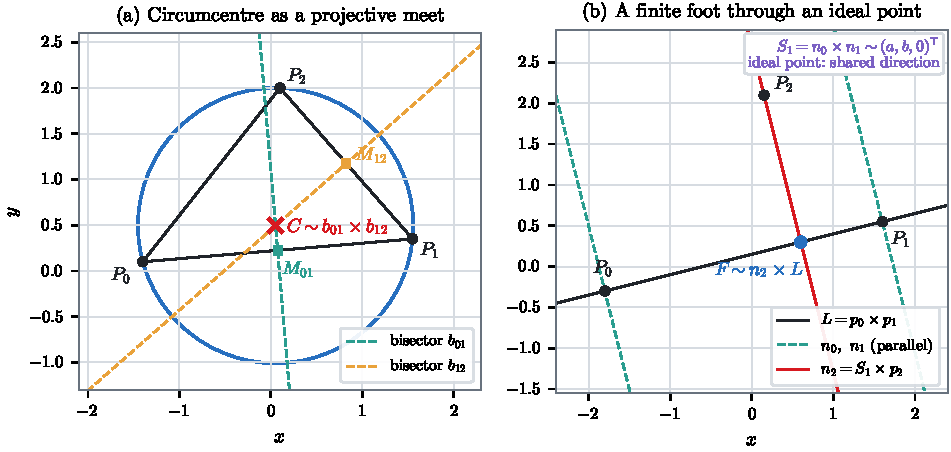
\includegraphics[width=\textwidth]{figures/projective_constructions.pdf}
  \caption[Two uses of homogeneous incidence]{Two uses of homogeneous incidence. (a) Euclidean perpendicular
  directions define projective bisector lines whose meet is the circumcentre.
  (b) The perpendiculars $n_0,n_1$ through $P_0$ and $P_1$ are parallel and meet
  at the ideal point $S_1$. The join of $S_1$ with $P_2$ is the perpendicular
  through $P_2$, whose finite intersection with the base line is the foot $F$.
  The symbol $\sim$ denotes equality up to a non-zero factor.}
  \label{fig:projective}
\end{figure}

\subsection{Perpendicular transport through an ideal point}

Suppose $L=p_0\times p_1=(a,b,c)^{\T}$. Its Euclidean normal direction is
$(a,b)$, so the corresponding ideal point is
\begin{equation}
  I_{\perp}=(a,b,0)^{\T}.
\end{equation}
The perpendiculars through $P_0$ and $P_1$ are $n_0=p_0\times I_{\perp}$ and
$n_1=p_1\times I_{\perp}$. Their meet $S_1=n_0\times n_1$ is again $I_{\perp}$
up to scale, because parallel lines meet at the ideal point encoding their
common direction. The perpendicular through any third point $P_2$ and its foot
are therefore
\begin{equation}
  n_2=S_1\times p_2,
  \qquad
  f=n_2\times L.
  \label{eq:perpendicular-foot}
\end{equation}
The source exercise deliberately constructs $S_1$ as the intersection of the
first two perpendiculars before reusing it. Algebraically, one could use the
direction $I_\perp$ directly. Pedagogically, the longer route is valuable
because it makes the projective closure visible: the ``missing'' intersection
of two parallel lines is a valid object rather than an exceptional return value.
A correct program should nevertheless verify that $S_1$ is ideal with a
scale-aware test, see \cref{eq:homogeneous-threshold} below. A short derivation
is given in \cref{app:perpendicular}.

\subsection{Isosceles apices as intersections of loci}\label{sec:isosceles}

Let $P_1\neq P_2$ be a fixed base of length $d=\norm{P_2-P_1}$, and let
$L_{\parallel}$ be the line through $P_0$ parallel to $P_1P_2$. An apex $Q$ on
$L_{\parallel}$ forms an isosceles triangle $P_1P_2Q$ whenever at least one of
the following conditions holds:
\begin{align}
  \norm{Q-P_1}&=\norm{Q-P_2}, \label{eq:iso1}\\
  \norm{Q-P_1}&=d, \label{eq:iso2}\\
  \norm{Q-P_2}&=d. \label{eq:iso3}
\end{align}
The first locus is the perpendicular bisector of $P_1P_2$; the second and third
are the circles $\Sph(P_1,d)$ and $\Sph(P_2,d)$. The number of apices depends
only on the ratio of the height $h$ of $L_\parallel$ above the base to the base
length.

\begin{proposition}[Isosceles apices on a parallel]\label{prop:isosceles}
Let $h$ be the signed distance of $L_{\parallel}$ from the line $P_1P_2$. If
$h=0$, every candidate triangle is degenerate. Otherwise the number $N$ of
distinct apices $Q\in L_\parallel$ for which $P_1P_2Q$ is isosceles is
\begin{equation}
  N=\begin{cases}
    5, & \abs{h}<d \text{ and } \abs{h}\neq\tfrac{\sqrt3}{2}d,\\
    3, & \abs{h}=\tfrac{\sqrt3}{2}d \text{ or } \abs{h}=d,\\
    1, & \abs{h}>d.
  \end{cases}
  \label{eq:isosceles-count}
\end{equation}
\end{proposition}

\begin{proof}
Choose coordinates with $P_1=(0,0)$, $P_2=(d,0)$, and $L_\parallel=\{y=h\}$.
\Cref{eq:iso1} gives $x=d/2$, i.e.\ exactly one apex for every $h$, because the
bisector is perpendicular to $L_\parallel$. With $s=\sqrt{d^2-h^2}$,
\cref{eq:iso2} gives $x=\pm s$ and \cref{eq:iso3} gives $x=d\pm s$: two points
each if $\abs{h}<d$, one (tangency) if $\abs{h}=d$, and none if $\abs{h}>d$.
A point of $\Sph(P_1,d)$ coincides with a point of $\Sph(P_2,d)$ only if
$s=d-s$, i.e.\ $s=d/2$, which is equivalent to $\abs{h}=\tfrac{\sqrt3}{2}d$;
the common point is then $x=d/2$, the bisector apex, so three candidates merge
into one (the equilateral triangle) and $5-2=3$ distinct apices remain. For
$\abs{h}=d$ the points $x=0$, $x=d/2$, $x=d$ are distinct. No other coincidences
are possible, and $h\neq0$ guarantees non-degenerate triangles.
\end{proof}

The construction is more informative than directly solving a quadratic because
it retains the reason for each solution family, see \cref{fig:isosceles}. The
submitted program computes the circle intersections correctly but reports
neither tangency nor coincidence, so in the equilateral configuration the same
apex is drawn three times; the revised program in \cref{app:programs} labels
every apex with its locus and merges coincident ones.

\begin{figure}[htbp]
  \centering
  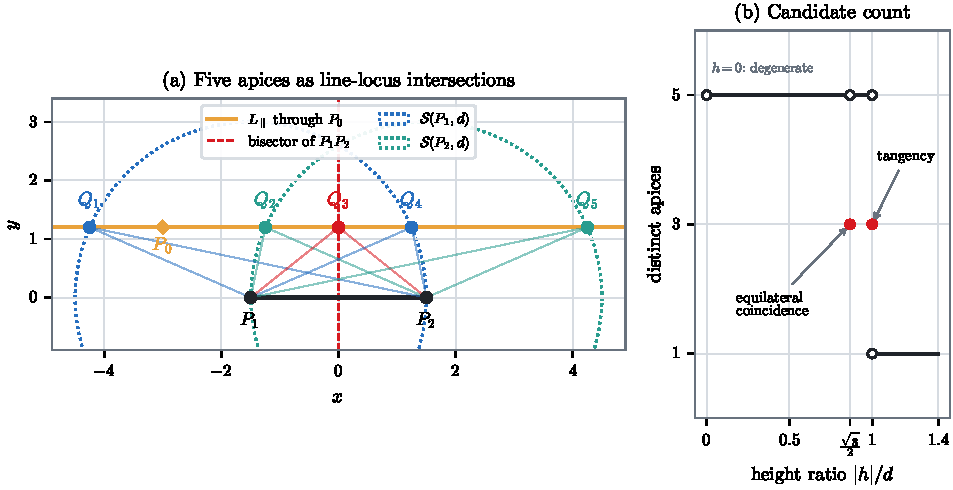
\includegraphics[width=\textwidth]{figures/isosceles_locus.pdf}
  \caption[Isosceles apices as line--locus intersections]{(a) The five generic isosceles apices on a line parallel to the fixed
  base: $Q_3$ lies on the perpendicular bisector, $Q_1,Q_4$ on $\Sph(P_1,d)$,
  and $Q_2,Q_5$ on $\Sph(P_2,d)$. (b) Number of distinct apices as a function of
  $\abs{h}/d$ (\cref{prop:isosceles}); open circles mark excluded values,
  filled dots the isolated values at the equilateral coincidence
  $\abs{h}/d=\sqrt3/2$ and at tangency $\abs{h}/d=1$; $h=0$ is degenerate.}
  \label{fig:isosceles}
\end{figure}

\FloatBarrier

% =============================================================================
\section{Conformal Geometric Algebra Layer}\label{sec:cga}
% =============================================================================

\subsection{Embedding Euclidean points}

The conformal model of $\R^3$ uses the geometric algebra $\GA$ generated by
$e_1,e_2,e_3,e_{+},e_{-}$ with $e_i^2=e_{+}^2=1$ and $e_{-}^2=-1$. The two null
vectors
\begin{equation}
  \einf=e_{-}+e_{+},\qquad \ezero=\tfrac12(e_{-}-e_{+}),
  \qquad
  \einf^2=\ezero^2=0,\quad \ezero\cdot\einf=-1,
\end{equation}
represent the point at infinity and the origin (CLUCalc: \texttt{einf},
\texttt{e0}). A Euclidean point $x\in\R^3$ is embedded as the null vector
\begin{equation}
  X=\mathcal{C}(x)=\ezero+x+\tfrac{1}{2}\norm{x}^2\einf .
  \label{eq:conformal-embedding}
\end{equation}
This normalisation gives $X^2=0$ and $X\cdot\einf=-1$; for a scaled point
$\lambda X$ the \emph{weight} is $-\lambda X\cdot\einf=\lambda$. Most
importantly, Euclidean distance is recovered through the inner product,
\begin{equation}
  X\cdot Y=-\tfrac{1}{2}\norm{x-y}^2 .
  \label{eq:cga-distance}
\end{equation}
Thus metric information that was external to the projective carrier becomes an
intrinsic bilinear relation of the conformal space. For instance, the vector
$X-Y$ satisfies $Z\cdot(X-Y)=\frac12(\norm{z-y}^2-\norm{z-x}^2)$ for every point
$Z$, so it represents the bisector plane $\bis(x,y)$ in IPNS.

There are two common representation conventions. In OPNS an object is the outer
product of points lying on it; in IPNS the dual object acts as a linear
constraint. With the dual $A^*=AI^{-1}$, $I=e_1e_2e_3e_{+}e_{-}$, the meet of two
OPNS objects can be written as
\begin{equation}
  A\cap B=\left(A^*\wedge B^*\right)^* .
  \label{eq:cga-meet}
\end{equation}
Signs and scales depend on conventions, but the geometric type of the result
does not. The CLUCalc expression \texttt{*(*A \^{} *B)} is the software-level
form of \cref{eq:cga-meet}. \Cref{tab:cga-primitives} lists the primitives used
in the three CLUCalc programs.

\begin{table}[H]
  \centering
  \caption[Conformal primitives]{Conformal primitives used in the CLUCalc programs. $C$ is the
  normalised conformal point of a centre $c$, $r$ a radius, $n$ a unit normal,
  and $\delta$ the signed distance of a plane from the origin.}
  \label{tab:cga-primitives}
  \small
  \begin{tabularx}{\textwidth}{@{}>{\raggedright\arraybackslash}p{27mm}p{44mm}Y@{}}
    \toprule
    Primitive & Representation & Geometric meaning \\
    \midrule
    Point & $X=\ezero+x+\tfrac12\norm{x}^2\einf$ & Null vector for $x\in\R^3$. \\
    Sphere (IPNS) & $s=C-\tfrac12r^2\einf$ & $X\cdot s=0$ iff $\norm{x-c}=r$. \\
    Plane (IPNS) & $\pi=n+\delta\einf$ & $X\cdot\pi=0$ iff $n\cdot x=\delta$. \\
    Bisector (IPNS) & $m=X_1-X_2$ & Points equidistant from $x_1$ and $x_2$. \\
    Plane (OPNS) & $X_1\wedge X_2\wedge X_3\wedge\einf$ & Plane through three points (\texttt{Bodenplatte}). \\
    Line (OPNS) & $X_1\wedge X_2\wedge\einf$ & Circle through two points and infinity. \\
    Circle (OPNS) & $X_1\wedge X_2\wedge X_3$ & Circle through three points. \\
    Point pair (OPNS) & $P=X_+\wedge X_-$ & Two real, one double, or two imaginary points. \\
    \bottomrule
  \end{tabularx}
\end{table}

The point-pair type is especially useful. A sphere--sphere--plane intersection
does not force a program to choose a solution; it returns one object encoding
both. Its square classifies the pair: $P\cdot P>0$ for two real points,
$P\cdot P=0$ for a tangent (double) point, and $P\cdot P<0$ for an imaginary
pair. The CLUCalc programs factorise a real pair with the formula
\begin{equation}
  P_{\pm}=\frac{\pm\sqrt{P\cdot P}+P}{\einf\cdot P},
  \label{eq:pointpair-formula}
\end{equation}
where the division is multiplication by the inverse vector
$(\einf\cdot P)^{-1}$, and then ``normalise'' by the \emph{multiplication}
$N_\pm=P_\pm\,(-P_\pm\cdot\einf)$. The following lemma, proved in
\cref{app:pointpair}, explains why this works and what it hides.

\begin{lemma}[Point-pair factorisation]\label{lem:pointpair}
Let $P=\lambda\,X\wedge Y$ with normalised points $X\neq Y$ and
$\lambda\in\R\setminus\{0\}$. Then $P\cdot P=\lambda^2(X\cdot Y)^2>0$ and
\begin{equation}
  \{P_+,P_-\}=\{-X,\,-Y\},
  \qquad
  P_+=\begin{cases}-Y,&\lambda>0,\\ -X,&\lambda<0.\end{cases}
\end{equation}
\end{lemma}

Two consequences matter for the audit. First, both extracted points have weight
exactly $-1$, so the multiplication by $-P_\pm\cdot\einf=-1$ coincides with the
correct division by the weight --- but only because the weight has modulus one.
Robust code divides. Second, \emph{which} point is returned first is not a
geometric property: it flips with the sign of $\lambda$, i.e.\ with the order of
the arguments and with the sign conventions of dual and meet. A program that
relies on ``the first point'' instead of an explicit selection rule inherits a
hidden convention dependence (\cref{sec:threelink,sec:audit}).

\subsection{Tripod from a three-sphere meet}\label{sec:tripod}

Let the fixed base points be $A,B,C$ and let the leg lengths be $r_A,r_B,r_C$.
The apex $S$ must satisfy
\begin{equation}
  \norm{S-A}=r_A,
  \qquad
  \norm{S-B}=r_B,
  \qquad
  \norm{S-C}=r_C.
  \label{eq:tripod-constraints}
\end{equation}
In CGA, the IPNS sphere vectors $s_A,s_B,s_C$ of \cref{tab:cga-primitives} meet
in a point pair,
\begin{equation}
  P_S=\left(s_A\wedge s_B\wedge s_C\right)^{*} \simeq S_+\wedge S_-,
  \label{eq:tripod-meet}
\end{equation}
which is the CLUCalc expression \texttt{*(*Kugel1 \^{} *Kugel2 \^{} *Kugel3)}
for the OPNS spheres $\texttt{Kugel}_i\simeq s_i^{*}$, up to sign and scale. When the centres lie in a common
ground plane, the two solutions are mirror images across that plane, since the
reflection preserves all three distances. Selecting the point with positive
height is a physical policy, not part of the meet itself.

The source task adds a fourth leg of prescribed length $r_4$. Its possible feet
form the circle in which the sphere around the selected apex cuts the ground
plane. The helper plane $\tau=A\wedge S_+\wedge S_-\wedge\einf$ --- the vertical
plane through $A$ and the apex, vertical because $S_+S_-$ is perpendicular to
the ground --- cuts this circle in two candidate feet, and the source program
chooses the one farther from $A$:
\begin{equation}
  \begin{gathered}
    K_4=\Sph(S_+,r_4)\cap\pi_{\mathrm{ground}},
    \qquad
    \{Q_{\mathrm{out}},Q_{\mathrm{in}}\}=K_4\cap\tau,\\
    Q_{\mathrm{out}}=\argmax_{Q\in K_4\cap\tau}\norm{Q-A}.
  \end{gathered}
  \label{eq:fourth-support}
\end{equation}
The report motivates the fourth leg by the instability of the tripod. This claim
can be made precise with the classical criterion of static stability.

\begin{definition}[Stability margin]\label{def:margin}
Let a structure rest on ground contacts $G_1,\dots,G_k$ and carry its load at a
point $S$. With $\proj$ the orthogonal projection onto the ground plane and
$\Omega=\conv\{G_1,\dots,G_k\}$ the support polygon, the stability margin is the
signed distance
\begin{equation}
  \mu=\begin{cases}
    \operatorname{dist}(\proj S,\partial\Omega), & \proj S\in\Omega,\\
    -\operatorname{dist}(\proj S,\Omega), & \proj S\notin\Omega.
  \end{cases}
  \label{eq:margin}
\end{equation}
The structure is statically stable if and only if $\mu>0$.
\end{definition}

With this definition the choice of the fourth foot becomes a policy with a
physical meaning,
$\sigma_{\mathrm{stab}}=\argmax_{Q}\mu\bigl(\conv\{A,B,C,Q\},S_+\bigr)$, which can
be compared with the distance heuristic of \cref{eq:fourth-support}
(\cref{sec:tripod-results}). The support polygon is computed with a standard
convex-hull algorithm \citep{deberg2008}. The whole construction is a good example
of the full pipeline: the algebra produces a circle and a point pair; the
application attaches a stability criterion to the pair.

\begin{figure}[htbp]
  \centering
  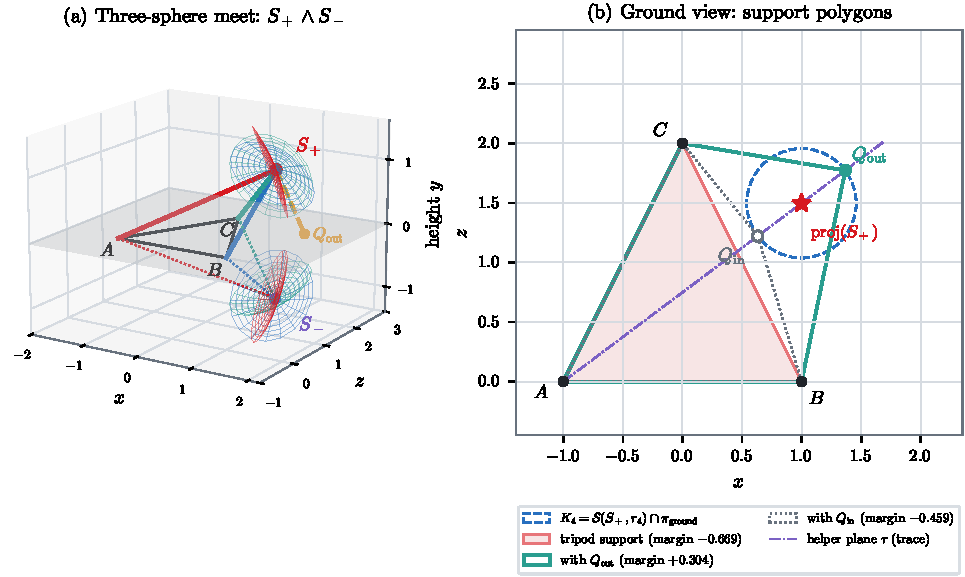
\includegraphics[width=\textwidth]{figures/tripod_construction.pdf}
  \caption[Tripod construction and support polygons]{Tripod construction. (a) Patches of the three leg spheres around
  their two common points: the meet is the point pair $S_+\wedge S_-$, whose
  points are mirror images in the ground plane; the upper point $S_+$ is
  selected and the fourth leg ends at $Q_{\mathrm{out}}$. (b) Ground view: the
  projection of $S_+$ lies outside the support triangle $ABC$ (negative margin);
  of the two feet on the circle $K_4$ cut out by the helper plane $\tau$, only
  $Q_{\mathrm{out}}$ yields a support polygon containing the projected apex.}
  \label{fig:tripod}
\end{figure}

\subsection{Two-link inverse kinematics}\label{sec:twolink}

Consider a shoulder at $O$, a target $T$, and link lengths $\ell_1,\ell_2$. The
elbow $E$ must lie on both link spheres:
\begin{equation}
  \norm{E-O}=\ell_1,
  \qquad
  \norm{E-T}=\ell_2.
  \label{eq:two-link-constraints}
\end{equation}
In three dimensions their intersection is generally a circle. A helper plane
through $O$ and $T$ fixes the intended motion plane, and the circle--plane meet
is a point pair $E_+\wedge E_-$. This mirrors the CLUCalc source directly, which
uses the vertical plane through $O$, the point $Z=(0,1,0)$, and $T$
(\texttt{U\^{}Z\^{}A\^{}einf}). That plane is undefined when $T$ lies on the vertical axis through $O$, a degeneracy that the
revised program handles with a fallback direction.

In a two-dimensional chart of the helper plane, let $d=\norm{T-O}$,
$u=(T-O)/d$, and let $u_{\perp}$ be a unit vector perpendicular to $u$ in that
plane. Then
\begin{equation}
  a=\frac{\ell_1^2-\ell_2^2+d^2}{2d},
  \qquad
  h=\sqrt{\ell_1^2-a^2},
  \qquad
  E_{\pm}=O+a u\pm h u_{\perp}.
  \label{eq:two-link-solutions}
\end{equation}
Real solutions exist exactly when
\begin{equation}
  \abs{\ell_1-\ell_2}\le d\le\ell_1+\ell_2 .
  \label{eq:reachability}
\end{equation}
Strict inequalities give two branches, equality gives a tangent (fully
stretched or folded) configuration, and violation gives no real elbow. A rule
such as ``choose the greater vertical coordinate'' should only be applied after
this classification; the submitted program lets its sliders reach targets with
$d>2$ and passes the resulting imaginary pair to the square root.

\subsection{Three-link arm: an isosceles trapezoid}\label{sec:threelink}

The third program moves an end point $T$ with three unit links $O\to E_1\to
E_2\to T$. Its construction is less obvious than its report suggests. It first
intersects the line $OT$ with the sphere $\Sph(T,1)$, which gives the two
auxiliary points $W_\pm=T\pm u$, $u=(T-O)/d$. It then intersects the bisector
plane of $O$ and the first auxiliary point with $\Sph(O,1)$, the bisector plane
of $O$ and the second auxiliary point with $\Sph(T,1)$, and cuts both circles
with the helper plane $\Pi$. The following proposition identifies the result.

\begin{proposition}[Three-link construction]\label{prop:trapezoid}
Let $0<d=\norm{T-O}\le 3$, let $u_\perp$ be the upward unit vector perpendicular
to $u$ in $\Pi$, and let $E_1$, $E_2$ be the upper points of
\begin{equation}
  \bis(O,W_-)\cap\Sph(O,1)\cap\Pi
  \qquad\text{and}\qquad
  \bis(O,W_+)\cap\Sph(T,1)\cap\Pi .
  \label{eq:trapezoid-construction}
\end{equation}
Then, with $h=\sqrt{1-(d-1)^2/4}$,
\begin{equation}
  E_1=O+\tfrac{d-1}{2}\,u+h\,u_\perp,
  \qquad
  E_2=O+\tfrac{d+1}{2}\,u+h\,u_\perp=E_1+u .
  \label{eq:trapezoid}
\end{equation}
Hence $\norm{E_1-O}=\norm{E_2-E_1}=\norm{T-E_2}=1$: the chain $OE_1E_2T$ is an
isosceles trapezoid with $E_1E_2\parallel OT$, symmetric with respect to
$\bis(O,T)$, and $E_1$ is the mirror image of $E_2$ in $\bis(O,T)$. The first
set in \cref{eq:trapezoid-construction} is undefined at $d=1$, where $W_-=O$.
\end{proposition}

The proof (\cref{app:trapezoid}) reduces to the observation that $\bis(O,wu)$
is the plane $\{x:(x-O)\cdot u=w/2\}$. Three consequences follow.

\emph{The program is correct, but for a non-obvious reason.} The auxiliary
points $W_\pm$ are not wrists of the arm; they only position the two bisector
planes. The arm itself is the trapezoid of \cref{eq:trapezoid}, visualised in
\cref{fig:kinematics}(b).

\emph{Correctness depends on the order of the extracted pair.} If the
factorisation returns $W_\pm$ in the opposite order --- which, by
\cref{lem:pointpair}, is a matter of sign conventions --- the program intersects
$\bis(O,W_+)$ with $\Sph(O,1)$ instead. The resulting crossed chain exists only
for $d\le1$, so a fraction $1-1/27\approx96.3\,\%$ of the reachable ball
$\norm{T-O}\le3$ would be lost.

\emph{The point $d=1$ is a representation singularity.} At $d=1$ the arm is
regular ($h=1$), yet $W_-=O$ and the IPNS bisector $O-W_-$ is the zero vector.
Near $d=1$ the vector $O-W_-$ is obtained by cancellation, and rounding errors
of order $\varepsilon_{\mathrm{mach}}$ tilt the bisector plane by an angle of order
$\varepsilon_{\mathrm{mach}}/\abs{d-1}$ (\cref{app:epsilon}). The revised
construction avoids $W_-$ altogether: $W_+$ is selected explicitly as the
auxiliary point farther from $O$ (it satisfies $\norm{W_+-O}=d+1\ge1$), $E_2$ is
obtained from one circle--plane meet, and $E_1$ by the reflection versor
\begin{equation}
  E_1=-\,m\,E_2\,m^{-1},\qquad m=O-T,
  \label{eq:reflection}
\end{equation}
where $m$ is the IPNS bisector plane of $O$ and $T$. Reflections preserve the
weight of a conformal point, so $E_1$ is again normalised. The revised
construction is exact for all $0<d\le3$; its only remaining singularities are
geometric: the direction $u$ is undefined at $d=0$, and the two branches merge
at full extension $d=3$.

\begin{figure}[htbp]
  \centering
  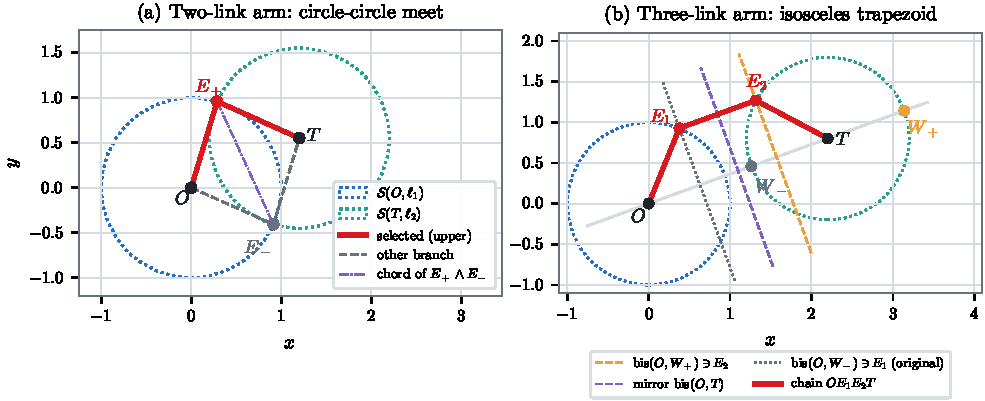
\includegraphics[width=\textwidth]{figures/kinematic_constructions.pdf}
  \caption[Two-link and three-link constructions]{Kinematic constructions in the helper plane. (a) Two unit circles
  meet at the two elbows $E_\pm$; the upper one is selected after both have been
  generated. (b) The three-link program: $E_2$ lies on $\Sph(T,1)$ and on the
  bisector of $O$ and $W_+=T+u$; $E_1$ is its mirror image in $\bis(O,T)$, so
  $OE_1E_2T$ is an isosceles trapezoid with three unit sides
  (\cref{prop:trapezoid}). The dotted plane $\bis(O,W_-)$ used by the original
  program passes through the same $E_1$; it degenerates when $d\to1$. Target
  distance $d\approx2.34$.}
  \label{fig:kinematics}
\end{figure}

\FloatBarrier

% =============================================================================
\section{A Unified Construction Pipeline}\label{sec:framework}
% =============================================================================

The planar and conformal tasks differ in dimension and metric content, but
their programs can be organised by the same six-stage pipeline shown in
\cref{tab:pipeline}. This organisation is the main synthesis of the paper.

\begin{table}[H]
  \centering
  \caption[Common construction pipeline]{Common pipeline for the two representation layers.}
  \label{tab:pipeline}
  \small
  \begin{tabularx}{\textwidth}{@{}>{\centering\arraybackslash}p{9mm}p{17mm}YY@{}}
    \toprule
    Stage & Question & Projective layer & Conformal layer \\
    \midrule
    1 & Encode & Lift $(x,y)$ to $(x,y,1)$; directions use $w=0$. & Lift $x$ to the null point $X=\mathcal C(x)$. \\
    2 & Construct & Form lines by point--point or point--direction joins. & Form spheres, planes, bisectors, lines, and circles as blades. \\
    3 & Intersect & Cross product of two line vectors. & Duality and outer product, \cref{eq:cga-meet}. \\
    4 & Factor & Dehomogenise a finite point or retain an ideal point. & Classify by $P\cdot P$; extract both points (\cref{lem:pointpair}); divide by the weight. \\
    5 & Select & Apply domain rules only if several objects remain. & Explicit policy $\sigma$: height, stability margin, continuity. \\
    6 & Validate & Incidence and Euclidean residuals. & Nullness, distance constraints, reality. \\
    \bottomrule
  \end{tabularx}
\end{table}

\subsection{Type before coordinates}

The first safety principle is to inspect the type and scale of an algebraic
result before converting it into ordinary coordinates. For a projective point
$p=(x,y,w)^{\T}$ the program should compare $\abs{w}$ with a scale-aware
tolerance,
\begin{equation}
  \abs{w}\le\tau\norm{p}_2 .
  \label{eq:homogeneous-threshold}
\end{equation}
If the condition holds, dividing by $w$ is unsafe and the result should be
reported as ideal or near-ideal. For a conformal point pair, the analogous step
is to classify the blade as real, tangent, or imaginary by the sign of $P\cdot
P$ relative to its scale before extraction.

This is more than defensive programming. The classification carries geometric
meaning. A circumcentre at infinity states that the defining points are
collinear. A tangent elbow pair states that the arm is fully stretched or
folded. An imaginary point pair states that the requested distances are
incompatible.

\subsection{Branch policy as an explicit function}

Let an intersection return a finite candidate set
$\mathcal S=\{q_1,\ldots,q_k\}$. A selection policy is a separate function
\begin{equation}
  \sigma(\mathcal S;\eta)\longrightarrow q_i ,
  \label{eq:selection-policy}
\end{equation}
where $\eta$ contains application context. Examples are height, distance from a
previous joint, support-polygon margin, or temporal continuity. Written this
way, the same construction can serve different applications without changes to
the intersection code.

The ``upper point'' policy of the source tasks is
$\sigma_{\mathrm{up}}(\mathcal S)=\argmax_{q\in\mathcal S}e_2^{\T}q$; it is
deterministic except when two candidates have equal height, which happens
exactly at tangency. The stability policy $\sigma_{\mathrm{stab}}$ of
\cref{sec:tripod} replaces a heuristic by a physical criterion. For an animated
arm, a continuity policy is usually better:
\begin{equation}
  \sigma_{\mathrm{cont}}(\mathcal S;q_{\mathrm{prev}})
  =\argmin_{q\in\mathcal S}\norm{q-q_{\mathrm{prev}}} .
  \label{eq:continuity-policy}
\end{equation}
It prevents a small target movement from causing an arbitrary elbow flip. In
every case the policy acts on \emph{named} candidates. \Cref{lem:pointpair} shows
why the order in which an algebra happens to return them must never act as an
implicit policy.

\subsection{Residuals as contracts}

Every stage should expose a postcondition. For projective incidence, a
scale-invariant residual is
\begin{equation}
  \rho_{\mathrm{inc}}(\ell,p)=
  \frac{\abs{\ell^{\T}p}}{\norm{\ell}_2\norm{p}_2} .
  \label{eq:incidence-residual}
\end{equation}
For a link or sphere constraint with centre $c$ and radius $r$ we use
\begin{equation}
  \rho_{\mathrm{dist}}(x;c,r)=\abs{\norm{x-c}_2-r} .
  \label{eq:distance-residual}
\end{equation}
For a configuration with several constraints, the maximum residual is a simple
and interpretable contract. A small residual does not prove that the problem is
well-conditioned, but a large residual immediately falsifies the result.

\begin{center}
\fbox{\begin{minipage}{0.94\textwidth}
\textbf{Reference procedure for a geometric intersection task}
\begin{enumerate}[label=\arabic*.,leftmargin=1.8em,topsep=3pt]
  \item Validate the input scale and reject undefined primitives.
  \item Embed the Euclidean inputs in the selected algebraic model.
  \item Construct the required loci from named geometric primitives.
  \item Compute the meet without selecting or discarding a branch.
  \item Classify the result as empty, tangent, multiple, finite, or ideal.
  \item Extract every real candidate and apply an explicit policy $\sigma$.
  \item Evaluate independent residuals and return the solution together with a
        diagnostic record.
\end{enumerate}
\end{minipage}}
\end{center}

\subsection{Geometric versus representation singularities}\label{sec:singularities}

The examples of \cref{sec:projective,sec:cga} suggest a distinction that is
useful when a construction misbehaves.

\begin{definition}\label{def:singularities}
Let a construction compute the solution $\Phi(x)$ of a geometric problem from
input data $x$ through a sequence of intermediate objects. A configuration $x^*$
is a \emph{geometric singularity} if the problem itself degenerates there: the
solution set changes cardinality or dimension, or $\Phi$ is not locally
Lipschitz at $x^*$. It is a \emph{representation singularity} of the
construction if $\Phi$ is regular at $x^*$ but an intermediate object of the
construction vanishes or becomes undefined.
\end{definition}

Collinear triangle vertices and a fully stretched arm are geometric
singularities: every formulation must report them, and near them every
formulation is sensitive, because the condition number of the problem itself is
large. The configuration $d=1$ of the three-link program is a representation
singularity: the trapezoid of \cref{prop:trapezoid} depends smoothly on $T$
there, but the bisector $\bis(O,W_-)$ does not exist. Near a representation
singularity the forward error of the construction grows although the problem is
well-conditioned. The remedy is a reformulation such as \cref{eq:reflection},
not more precision.

% =============================================================================
\section{Experimental Methodology}\label{sec:experiments}
% =============================================================================

\subsection{Implementation and reproducibility}

All experiments use Python~3.12, NumPy double precision, Matplotlib, and the
fixed random seed \ExperimentSeed. The script \texttt{code/generate\_figures.py}
creates every reported number, all table entries, and all plots from a clean
checkout; no value was transcribed by hand. The code consists of four modules:
\begin{itemize}
  \item \texttt{cga.py}: a self-contained implementation of $\GA$ with $32$
        coefficients per multivector, geometric, outer and inner products,
        inverse, dual $A^*=AI^{-1}$, and CLUCalc counterparts
        (\texttt{VecN3}, \texttt{SphereN3}, meet, point-pair factorisation);
  \item \texttt{geometry.py}: closed-form Euclidean and projective reference
        solutions of all six tasks, returning structured results
        (status, candidates, selection, residual);
  \item \texttt{homework\_cga.py}: line-by-line transcriptions of the three
        CLUCalc programs in their original and revised form;
  \item \texttt{tests/}: twelve unit tests, including the execution of the
        revised \texttt{libcfcg} programs against a headless stand-in of the
        library.
\end{itemize}
This yields a cross-implementation validation: the constructions come from the
source programs, while the residuals are evaluated by independent formulas.

\subsection{Experiment 1: projective covariance}

For each of \ProjectiveTrials{} trials, four affine points were sampled
uniformly from $[-2,2]^2$ and embedded with $w=1$. Two lines and their
intersection were computed by cross products. A random homography $H=I+0.22N$,
with standard normal entries in $N$, was accepted when $\abs{\det H}>0.15$ and
$\kappa_2(H)<50$. Points were transformed by $H$ and lines by $H^{-\T}$. The
per-trial error was the maximum of the transformed incidence residuals
\cref{eq:incidence-residual}, the angular disagreement between directly
recomputed joins and $H^{-\T}\ell$, and the angular disagreement between the
directly recomputed meet and $Hs$. The experiment deliberately does not test
the preservation of perpendicularity, because a general homography does not
preserve Euclidean angles.

\subsection{Experiment 2: constraints of the closed forms}

For the two-link arm with unit links, \TwoLinkTrials{} planar targets were
sampled uniformly by area in the annulus $0.05\le d\le1.95$, which avoids the
origin and the tangent outer boundary. The upper elbow of
\cref{eq:two-link-solutions} was selected and the maximum of the two link-length
residuals was recorded. For the three-link arm, \ThreeLinkTrials{} targets were
sampled in $0.05\le d\le2.95$, the trapezoid \cref{eq:trapezoid} was evaluated,
and the maximum error of the three link lengths was recorded. For
\cref{prop:isosceles}, \IsoTrials{} random configurations with base length at
least $0.2$ were drawn from $[-3,3]^2$; the number of apices found by the locus
construction was compared with \cref{eq:isosceles-count}, including the two
exceptional heights, and the isosceles residual was recorded.

\subsection{Experiment 3: tripod and support polygon}

The source tripod uses
\begin{equation}
  \begin{gathered}
    A=(-1,0,0),\qquad B=(1,0,0),\qquad C=(0,0,2),\\
    r_A=2.69,\qquad r_B=1.8,\qquad r_C=1.5,
  \end{gathered}
\end{equation}
with the second coordinate as height. Both sphere intersections were obtained
by the linear reduction of \cref{app:trilateration}, the positive-height branch
was selected, and the fourth foot of length $1.1$ was computed with
\cref{eq:fourth-support}. The maximum distance residual over the four legs was
recorded, and the stability margin \cref{eq:margin} was evaluated for the
tripod and for both candidate feet, assuming the load at the apex.

\subsection{Experiment 4: conditioning near singularities}\label{sec:conditioning}

Three limits were studied. For the circumcentre, the triangle
\begin{equation}
  P_0=(-1,0),\qquad P_1=(1,0),\qquad P_2=(0,h)
  \label{eq:thin-triangle}
\end{equation}
was evaluated for 21 logarithmically spaced altitudes from $10^{-1}$ to
$10^{-11}$. The centre solves the linear system $Mc=b$ with
$M=2\,[P_1-P_0,\ P_2-P_0]^{\T}$ and
$b=(\norm{P_1}^2-\norm{P_0}^2,\ \norm{P_2}^2-\norm{P_0}^2)^{\T}$; for this
triangle $\kappa_2(M)=2.5/h+O(h)$. Each coordinate was perturbed by independent
Gaussian noise of standard deviation $10^{-10}$ in 400 repetitions, and the
median relative centre error was recorded.

For the two-link arm, the target distance approached the tangent value $d=2$.
With the elbow height $h=\sqrt{1-(d/2)^2}$, the branch separation is $2h$,
while
\begin{equation}
  \abs{\frac{\mathrm dh}{\mathrm dd}}=\frac{d}{4h}
  \label{eq:elbow-sensitivity}
\end{equation}
diverges as $d\to2^-$.

For the three-link arm, targets $T=(1+\delta)u$ were generated for 20 random
directions $u$ and 27 values $\delta\in[10^{-14},10^{-1}]$. Both the original
and the revised CLUCalc construction were executed in the CGA engine, and the
median position error of $(E_1,E_2)$ relative to \cref{eq:trapezoid} was
recorded.

\subsection{Experiment 5: executing the CLUCalc programs}\label{sec:exp-cga}

The three CLUCalc programs were transcribed statement by statement, including
the point-pair formula \cref{eq:pointpair-formula} and the multiplicative
normalisation. For the two-link program, \CGATrials{} targets were sampled
uniformly by volume in the shell $0.05\le d\le1.95$; for the three-link
program, \CGATrials{} targets in $0.05\le d\le2.95$. The elbows of the original
and the revised transcription were compared with the closed forms
\cref{eq:two-link-solutions,eq:trapezoid}. To expose the ordering dependence
of \cref{lem:pointpair}, the three-link program was additionally executed with
the two auxiliary points interchanged, which emulates the opposite sign
convention. The tripod program was executed once in both versions.

% =============================================================================
\section{Results}\label{sec:results}
% =============================================================================

\subsection{Constraint validation}

\Cref{tab:validation} summarises the regular-case validation. All median
residuals are at the level of the unit roundoff $1.1\times10^{-16}$, and every
maximum remains below $10^{-13}$. The projective experiment has the largest
maximum because it composes a matrix inversion, two transformations, and
several cross products; the kinematic formulas evaluate only a few normalised
vector operations and square roots. The apex count predicted by
\cref{prop:isosceles} agreed with the locus construction in all \IsoTrials{}
random configurations and at both exceptional heights (\IsoMismatch{}
mismatches).

\begin{table}[H]
  \centering
  \caption[Residual validation]{Residual validation in double precision. Projective values combine
  incidence and covariance errors; the isosceles value is the relative
  deviation from the nearest isosceles condition; the remaining values are
  absolute link or sphere-distance errors.}
  \label{tab:validation}
  \small
  \begin{tabularx}{\textwidth}{@{}Y r r r@{}}
    \toprule
    Experiment & Trials & Median residual & Maximum residual \\
    \midrule
    Projective join/meet covariance & \ProjectiveTrials & \ProjectiveMedian & \ProjectiveMaximum \\
    Isosceles apices (\cref{prop:isosceles}) & \IsoTrials & --- & \IsoMaximum \\
    Two-link distance constraints & \TwoLinkTrials & \TwoLinkMedian & \TwoLinkMaximum \\
    Three-link distance constraints & \ThreeLinkTrials & \ThreeLinkMedian & \ThreeLinkMaximum \\
    Tripod and fourth support & 1 & \TripodMaximum & \TripodMaximum \\
    \bottomrule
  \end{tabularx}
\end{table}

The results support the first two research questions. Cross products and
conformal meets both serve as a construction grammar, and explicit branch
selection does not compromise the constraints when it is applied after the full
solution set has been produced. The data do not establish that one algebra is
faster than the other; no timing comparison was attempted.

\subsection{Numerical tripod and static stability}\label{sec:tripod-results}

The selected upper apex and the two candidate feet are
\begin{equation}
  \begin{aligned}
    S_+&=\ApexCoordinates,\\
    Q_{\mathrm{out}}&=\FourthFootCoordinates,\qquad
    Q_{\mathrm{in}}=\InnerFootCoordinates .
  \end{aligned}
\end{equation}
The reflected apex $S_-$ has the same first and third coordinates and the
opposite height. The maximum residual across the three original legs and the
added $1.1$-unit leg is \TripodMaximum.

The stability margins answer the question that the distance heuristic leaves
open. With the load at the apex, the tripod alone has $\mu=\MarginTripod$: the
projected apex lies beyond the edge $BC$ of the support triangle, so the
structure tips over, which confirms the claim of the original report. Adding
$Q_{\mathrm{in}}$ still gives $\mu=\MarginIn$, whereas $Q_{\mathrm{out}}$ gives
$\mu=+\MarginOut$ (\cref{fig:tripod}b). For this geometry the heuristic ``farther
from $A$'' therefore coincides with the stability policy
$\sigma_{\mathrm{stab}}$, and it is the only admissible choice. This agreement
is a property of the data, not a theorem: in general, static stability depends
on the projection of the centre of mass, and structural stiffness on material
and joint properties. The algebra generates the feasible feet; the engineering
model decides which one is preferable.

\subsection{Behaviour near degeneracy}

\Cref{tab:conditioning} and \cref{fig:stability} answer the third research
question. As the altitude decreases, the circumcentre system becomes nearly
singular: $\kappa_2(M)$ grows like $h^{-1}$, and the median relative error of the
centre follows the same trend until it saturates at order one, when the
altitude reaches the noise level. The homogeneous construction still returns a
vector, and its incidence residual may remain small, but the dehomogenised
centre is no longer a reliable estimate of the unperturbed problem.

\begin{table}[H]
  \centering
  \caption[Circumcentre conditioning]{Circumcentre conditioning for selected triangle altitudes. Each
  median error is based on 400 perturbations with coordinate noise of standard
  deviation $10^{-10}$.}
  \label{tab:conditioning}
  \small
  \begin{tabular}{@{}r r r@{}}
    \toprule
    Altitude $h$ & $\kappa_2(M)$ & Median relative centre error \\
    \midrule
    \ConditionHeightA & \ConditionKappaA & \ConditionErrorA \\
    \ConditionHeightB & \ConditionKappaB & \ConditionErrorB \\
    \ConditionHeightC & \ConditionKappaC & \ConditionErrorC \\
    \ConditionHeightD & \ConditionKappaD & \ConditionErrorD \\
    \ConditionHeightE & \ConditionKappaE & \ConditionErrorE \\
    \bottomrule
  \end{tabular}
\end{table}

The two-link plot shows the same phenomenon in a different language. As the two
circles approach tangency, the elbow branches merge and their separation tends
to zero, while the derivative of the elbow height with respect to the target
distance diverges. A small target perturbation may therefore produce a large
change of the elbow height even though both link lengths remain satisfied to
machine precision.

The three-link experiment isolates the representation singularity. The error of
the original construction follows $\varepsilon_{\mathrm{mach}}/\abs{d-1}$ over
thirteen orders of magnitude and reaches \ThreeSingOrig{} at
$\abs{d-1}=10^{-7}$, while the revised construction stays below
\ThreeSingRevMax{} for every tested $\delta$ (\cref{fig:stability}c). Since
the trapezoid itself is well-conditioned near $d=1$, this amplification is
entirely a property of the formulation.

\begin{figure}[htbp]
  \centering
  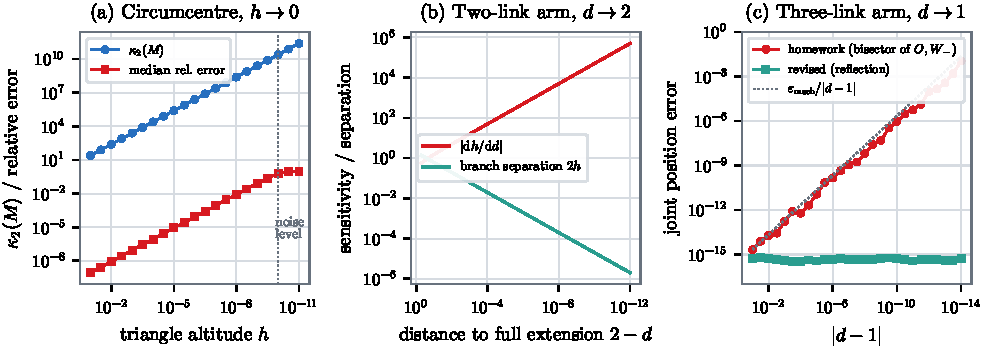
\includegraphics[width=\textwidth]{figures/stability_analysis.pdf}
  \caption[Geometric and representation singularities]{Three limits. (a) Geometric singularity: the circumcentre becomes
  sensitive as the triangle approaches collinearity. (b) Geometric singularity:
  the elbow branches merge at full extension while the derivative of their
  height diverges. (c) Representation singularity: the original three-link
  construction loses accuracy like $\varepsilon_{\mathrm{mach}}/\abs{d-1}$ near
  $d=1$, where the arm is regular; the reflection-based construction does not.}
  \label{fig:stability}
\end{figure}

\subsection{Audit of the source programs}\label{sec:audit}

\Cref{tab:cga-execution} reports the execution of the CLUCalc programs in the
CGA engine, and \cref{tab:audit} lists all observations together with the
revisions reproduced in \cref{app:programs}.

\begin{table}[H]
  \centering
  \caption[Execution of the CLUCalc programs in the CGA engine]{Execution of the CLUCalc programs in the independent CGA engine:
  maximum Euclidean deviation of the computed joints from the closed-form
  solutions.}
  \label{tab:cga-execution}
  \small
  \begin{tabularx}{\textwidth}{@{}>{\raggedright\arraybackslash}p{27mm}p{13mm}rY@{}}
    \toprule
    Program & Version & Max.\ error & Remark \\
    \midrule
    Hausaufgabe 1 (tripod) & original & \CGATripodOrig & Apex and outer foot correct; the selection is bypassed when drawing. \\
                           & revised  & \CGATripodRev  & Selected points used throughout. \\
    Hausaufgabe 2 (two-link) & original & \CGATwoOrig & \CGATrials{} targets; correct off the vertical axis. \\
                             & revised  & \CGATwoRev  & Adds reachability test and plane fallback. \\
    Hausaufgabe 3 (three-link) & original & \CGAThreeOrig & Median \CGAThreeOrigMedian; the maximum occurs close to $d=1$ (\CGAThreeBad{} target with error $>10^{-12}$). With interchanged auxiliary points, \CGAThreeSwapFail\,\% of the targets become unreachable (theory for this shell: $96.1\,\%$). \\
                               & revised  & \CGAThreeRev & Uniform accuracy; largest errors close to full extension $d\to3$. \\
    \bottomrule
  \end{tabularx}
\end{table}

\begin{table}[H]
  \centering
  \caption[Audit of the submitted programs]{Observations on the submitted programs and the corresponding
  revisions.}
  \label{tab:audit}
  \footnotesize
  \begin{tabularx}{\textwidth}{@{}>{\raggedright\arraybackslash}p{21mm}YY@{}}
    \toprule
    Program & Observation and consequence & Revision \\
    \midrule
    Aufgabe 1 & Collinearity test with the absolute threshold $\abs{\Delta}<10^{-3}$; its outcome depends on the unit of the data. & Relative test \cref{eq:relative-collinearity}; centre classified by \cref{eq:homogeneous-threshold}; residual reported. \\
    Aufgabe 2 & The perpendiculars are called ``bisectors''; the ideal point $S_1$ is printed but not verified. & Naming corrected; scale-aware ideal test; residuals of the foot. \\
    Aufgabe 4 & Tangency and coincidences are not reported, so the equilateral apex is drawn three times; $P_0$ on the base line is not detected; fixed drawing window. & Classification per locus (\cref{prop:isosceles}), merging of coincident apices, degeneracy test, data-driven window. \\
    Hausaufgabe 1 & The apex \texttt{Spitze} is selected, but legs and the fourth sphere use \texttt{N\_Pp2}, and the last leg is drawn to \texttt{N\_Pp4} instead of \texttt{AußenPunkt}; whether this is correct depends on the ordering of the pair (\cref{lem:pointpair}). Duplicated header, non-ASCII identifiers. & Selected points used throughout; header cleaned; ASCII identifiers. \\
    Hausaufgabe 2 & Helper plane undefined for targets on the vertical axis; sliders reach $d>2$ without a reachability test. & Fallback direction; classification by the sign of $P\cdot P$ before factorisation. \\
    Hausaufgabe 3 & Correctness relies on the implicit order of \texttt{N\_Pp1}, \texttt{N\_Pp2}; representation singularity at $d=1$. & $W_+$ chosen by distance; $E_1$ by the reflection \cref{eq:reflection}. \\
    All CLUCalc & Normalisation by multiplication with $-X\cdot\einf$; correct only because the weight is $\pm1$. & Division by the weight $-X\cdot\einf$. \\
    \bottomrule
  \end{tabularx}
\end{table}

Two findings deserve emphasis. First, none of the observations changes the
geometric idea of a program; they concern selection, classification, and
conventions --- exactly the stages 4--6 of \cref{tab:pipeline} that the
exercises leave implicit. Second, the most instructive defect, the
representation singularity of Hausaufgabe~3, is invisible in interactive use:
the slider grid never hits $d=1$ exactly, and the error exceeds $10^{-12}$ only in
a tiny neighbourhood of that sphere. It is found only by a systematic
experiment or by a proof.

% =============================================================================
\section{Discussion}\label{sec:discussion}
% =============================================================================

\subsection{What is genuinely unified?}

The most compelling common feature of the tasks is not a particular formula but
the conversion of a verbal construction into intersections of named loci. The
circumcentre is the intersection of bisectors. The isosceles apices are
intersections of a line with a bisector or with circles. The tripod apex is the
intersection of three spheres. The elbow is the intersection of two link
spheres and a helper plane, and the three-link chain is obtained from two
bisector planes. Once the loci are explicit, solution multiplicity and
degeneracy follow from their geometry, as \cref{prop:isosceles,prop:trapezoid}
illustrate.

Homogeneous coordinates and CGA supply compatible algebraic habits: objects are
represented up to scale, joins are outer constructions, meets are dual
constructions, and ideal elements close the incidence system. CGA goes further
by internalising Euclidean distance and representing round primitives directly.
The relation should be understood as a progression, not an identity: $\PP^2$ is a
three-coordinate projective model of planar incidence, whereas $\GA$ is a
Clifford algebra over the five-dimensional space $\R^{4,1}$ of signature
$(4,1)$.

\subsection{The value of visible multiplicity}

Ordinary application code often returns one answer because a downstream
component expects one. The source tasks are more instructive: they make the
pair of sphere intersections or elbow positions visible before choosing. This
has three benefits. It prevents silent branch loss. It makes singularity
detection natural, because two branches coalesce at tangency. And it supports
different policies without changing the geometric solver: an interactive
visualisation may choose the upper point, a trajectory the nearest previous
joint, and a structural design the foot with the largest stability margin.

The isosceles example generalises the lesson beyond pairs: there are up to five
candidates because there are three distinct ways in which a triangle with a
fixed base can be isosceles, and \cref{prop:isosceles} states exactly when they
merge. The audit adds a complementary lesson: visible multiplicity is only safe
if the candidates are \emph{named} by geometry, not by the order in which the
algebra returns them.

\subsection{Where the algebra does not help automatically}

Five limitations are important.

\textbf{Numerical scale remains important.} Homogeneous objects can be multiplied
by arbitrary non-zero scalars. Without normalisation, residual thresholds have
no consistent meaning and intermediate coefficients can overflow or underflow.
Scale-invariant tests such as \cref{eq:relative-collinearity,eq:incidence-residual}
should be preferred.

\textbf{Degenerate geometry remains degenerate.} Representing an ideal
circumcentre is mathematically elegant, but a program that needs a finite radius
must still stop. Likewise, CGA encodes a tangent point pair compactly, but the
branch derivative is still singular.

\textbf{Constructions can create their own singularities.} The three-link program
shows that an algebraically correct construction may route the computation
through an object that degenerates where the problem does not. Such
representation singularities are avoided by choosing intermediate objects that
exist throughout the domain, as in \cref{eq:reflection}.

\textbf{Selection is not solved by representation.} CGA returns both elbows, but
it cannot decide which one is collision-free or comfortable without additional
constraints. The choice belongs to the application model.

\textbf{A richer algebra has computational overhead.} Cross products of
three-vectors are inexpensive. General conformal multivector operations evaluate
many more coefficients than a specialised Euclidean formula. Sparse typed
implementations mitigate this cost \citep{hildenbrand2013,low2023}, but the
present experiments do not compare execution time or memory, and no performance
claim is made.

\subsection{Improvements for production implementations}

The educational programs can be developed into robust software through five
concrete changes, all of which are realised in the revised programs of
\cref{app:programs}:
\begin{enumerate}
  \item Replace fixed absolute tolerances by scale-aware thresholds.
  \item Return structured results containing status, all candidates, the
        selected candidate, and residuals.
  \item Select candidates by explicit, named policies; use continuity-aware
        selection for time-dependent targets.
  \item Guard orientation, tangency, and reality predicates, using adaptive
        precision when a discrete decision is numerically ambiguous.
  \item Add property-based tests under rigid motions, scalings, and admissible
        projective transformations of the incidence subproblems.
\end{enumerate}
A possible result record is
\begin{equation}
  \texttt{ConstructionResult}
  = (\texttt{status},\texttt{candidates},\texttt{selected},
     \texttt{residual},\texttt{info}),
\end{equation}
as implemented in \texttt{geometry.py}. Such a record makes the diagnostic
information part of the public interface rather than console output that a
caller may ignore.

\subsection{Threats to validity}

The study uses synthetic configurations and low-dimensional mechanisms. The
residual experiments show that the formulas were implemented consistently, not
that they solve all robotics or structural-design problems. Joint limits,
obstacles, uncertainty, force transmission, and dynamic effects are absent.
The three-link construction selects one symmetric family of configurations and
is not a complete parameterisation of the redundancy.

The CLUCalc programs were not run in CLUCalc itself but in an independent
implementation of $\GA$. This checks the mathematics of every statement, but
software-specific conventions --- the sign of the dual, the definition of the
inner product, rendering --- may differ. For this reason, conclusions that depend
on such conventions are stated as dependencies (for instance, on the ordering of
a point pair) rather than as failures of the submitted programs. Likewise, the
Python programs were executed against a stand-in of \texttt{libcfcg} that
implements only the interface they use. Finally, the perturbation study examines
three representative singularities rather than a complete error analysis of all
constructions.

% =============================================================================
\section{Conclusion}\label{sec:conclusion}
% =============================================================================

This paper transformed two groups of geometry exercises into one computational
study. The homogeneous layer showed how points, lines, directions, joins, and
meets provide a closed language for planar incidence; its most memorable object
is the ideal point shared by parallel perpendiculars. The conformal layer
extended the same construction-oriented thinking to distance geometry: spheres
meet in circles or point pairs, helper planes reduce solution families, and
robot joints emerge as intersections of geometric constraints.

The synthesis led to a six-stage pipeline: encode, construct, intersect, factor,
select, and validate. Separating the selection stage was decisive. ``Upper
elbow'' and ``outer support'' are useful policies, but they are not properties of
the intersection algebra; for the tripod the latter could be justified by a
stability margin, which turned a heuristic into a criterion. Keeping all
candidates until selection preserves the geometry and makes tangency and
non-uniqueness visible --- provided the candidates are identified by geometry
rather than by the order in which an algebra returns them.

The numerical experiments confirmed the constraints at machine precision for
thousands of regular configurations. They also demonstrated the central caution
in two forms. An elegant representation does not cure an ill-conditioned
problem: circumcentres remain unstable near collinearity and elbows near
tangency. Conversely, an elegant construction can itself be unstable where the
problem is harmless, as the representation singularity of the three-link
program shows; there, a better formulation --- a single reflection --- removes the
defect completely. The proper conclusion is not to abandon lifted models, but to
pair them with classification, scale-aware tolerances, residuals, and explicit
diagnostics, and to test constructions against independent formulas.

For future work, the framework can be extended in three directions: a typed
implementation that exposes point pairs and ideal points as first-class return
types; continuous branch tracking with joint limits and obstacle constraints;
and a comparative benchmark between specialised Euclidean formulas and sparse
CGA code that measures not only speed but also implementation complexity,
invariance, and failure behaviour near singularities. Those extensions would
preserve what is most valuable in the present tasks: geometry remains visible
in the code.

% =============================================================================
\appendix
\section{Selected Derivations}\label{app:derivations}
% =============================================================================

\subsection{Why the projective perpendicular construction works}\label{app:perpendicular}

Let $L=(a,b,c)^{\T}$ be a finite line, i.e.\ $(a,b)\neq(0,0)$. Its direction is
$(-b,a)$ and its normal direction is $(a,b)$. The ideal point
$I_{\perp}=(a,b,0)^{\T}$ therefore encodes the direction of every line
perpendicular to $L$. For a finite point $p$, the join $n=p\times I_{\perp}$ is
incident with $p$ and with that ideal point; hence it is precisely the
perpendicular through $p$. The foot $f=(p\times I_{\perp})\times L$ is incident
with both lines, and for $p=(x,y,1)^{\T}$ its third coordinate is
$f_3=-(a^2+b^2)\neq0$, so the foot is always finite. No slope is used, so vertical and horizontal base lines require
no special branch.

\subsection{Linear reduction of the three-sphere intersection}\label{app:trilateration}

For centres $c_i$ and radii $r_i$, an intersection point $x$ satisfies
$\norm{x-c_i}^2=r_i^2$. Subtracting the first equation from the second and third
eliminates $\norm{x}^2$:
\begin{equation}
  2(c_i-c_1)^{\T}x
  =r_1^2-r_i^2+\norm{c_i}^2-\norm{c_1}^2,
  \qquad i\in\{2,3\}.
  \label{eq:trilateration-linear}
\end{equation}
For non-collinear centres these two planes meet in a line
$x=x_0+t\,n$, $n\parallel(c_2-c_1)\times(c_3-c_1)$. Substituting into the
first sphere gives a quadratic in $t$ with zero, one, or two real roots. In the
conformal representation, the same reduction is captured by the meet of three
spheres, whose result type is already a point pair. The reference implementation
uses \cref{eq:trilateration-linear}, which provides an independent check of the
conformal construction.

\subsection{Two-circle intersection formula}

Choose coordinates with $O=0$ and write the target as $T=du$. Decompose an elbow
as $E=au+bu_{\perp}$. The two length equations are
\begin{equation}
  a^2+b^2=\ell_1^2,
  \qquad
  (a-d)^2+b^2=\ell_2^2 .
\end{equation}
Subtracting them yields $a=(\ell_1^2-\ell_2^2+d^2)/(2d)$; substitution gives
$b=\pm\sqrt{\ell_1^2-a^2}$. The two signs are the two point-pair branches. If the
radicand is zero, the circles are tangent; if it is negative, the pair is
imaginary and the target is unreachable. A short computation shows
$\ell_1^2-a^2\ge0$ if and only if \cref{eq:reachability} holds.

\subsection{Proof of Lemma~\ref{lem:pointpair}}\label{app:pointpair}

Write $P=\lambda P_0$ with $P_0=X\wedge Y$ and let $s_0=-X\cdot Y=\frac12\norm{x-y}^2>0$.
For null vectors, $P_0\cdot P_0=(X\cdot Y)^2-X^2Y^2=s_0^2$, hence
$P\cdot P=\lambda^2s_0^2$ and $\sqrt{P\cdot P}=\abs{\lambda}s_0$. Moreover
$\einf\cdot P_0=(\einf\cdot X)Y-(\einf\cdot Y)X=X-Y$, and
$(X-Y)^2=-2X\cdot Y=2s_0$, so $(X-Y)^{-1}=(X-Y)/(2s_0)$. Using
$(X\wedge Y)Z=(X\wedge Y)\cdot Z=X(Y\cdot Z)-Y(X\cdot Z)$ for $Z\in\{X,Y\}$
(the outer part vanishes because $Z$ is contained in $X\wedge Y$), we obtain
$P_0X=-s_0X$ and $P_0Y=s_0Y$. Therefore
\begin{equation}
  (s_0+P_0)(X-Y)=s_0X-s_0Y-s_0X-s_0Y=-2s_0Y,
  \qquad
  (-s_0+P_0)(X-Y)=-2s_0X,
\end{equation}
and division by $2s_0$ gives $(\pm s_0+P_0)(\einf\cdot P_0)^{-1}=-Y$ and $-X$,
respectively. For $\lambda>0$ the factors $\lambda$ cancel and
$P_+=-Y$, $P_-=-X$. For $\lambda<0$ we have $\abs{\lambda}s_0+\lambda P_0=
\lambda(-s_0+P_0)$, so the roles are interchanged: $P_+=-X$, $P_-=-Y$. In both
cases $-P_\pm\cdot\einf=-1$, i.e.\ the weight is $-1$. \qed

\subsection{Proof of Proposition~\ref{prop:trapezoid}}\label{app:trapezoid}

Let $O=0$ and $W=wu$ with $w\neq0$. Then $\norm{x-W}^2-\norm{x}^2=w^2-2w\,x\cdot u$,
so $\bis(0,W)=\{x: x\cdot u=w/2\}$. For $W_+=(d+1)u$ the bisector is the plane
$x\cdot u=(d+1)/2$; its points on $\Sph(T,1)$ have axial distance
$\abs{(d+1)/2-d}=\abs{d-1}/2$ from $T$ and hence the transverse radius
$h=\sqrt{1-(d-1)^2/4}$. For $W_-=(d-1)u$, which is non-zero if and only if
$d\neq1$, the bisector is $x\cdot u=(d-1)/2$, and its points on $\Sph(0,1)$ have
the same transverse radius $h$. Within the helper plane $\Pi=\operatorname{span}
\{u,u_\perp\}$ the upper points are those of \cref{eq:trapezoid}, so
$E_2-E_1=u$ and all three links have unit length. The reflection in
$\bis(0,T)=\{x:x\cdot u=d/2\}$ maps the axial coordinate $(d+1)/2$ to
$d-(d+1)/2=(d-1)/2$ and preserves the transverse part; hence it maps $E_2$ to
$E_1$. The points are real if and only if $(d-1)^2\le4$, i.e.\ $d\le3$. In CGA,
the reflection of a conformal point $X$ in the IPNS plane $m$ is $X\mapsto-mXm^{-1}$,
and $m=O-T$ represents $\bis(O,T)$ by \cref{eq:cga-distance}; this gives
\cref{eq:reflection}. If the auxiliary points are interchanged, the upper points
of $\bis(0,W_+)\cap\Sph(0,1)$ and $\bis(0,W_-)\cap\Sph(T,1)$ have the transverse
radius $\sqrt{1-(d+1)^2/4}$, which is real only for $d\le1$. \qed

\subsection{Error growth near the representation singularity}\label{app:epsilon}

In floating-point arithmetic the auxiliary point is computed as
$\widehat W_-=W_-+\eta$ with $\norm{\eta}\le c\,\varepsilon_{\mathrm{mach}}$ for a
modest constant $c$, because $T$ and $u$ have norms of order one. The bisector of
$O$ and $\widehat W_-$ has the normal $\widehat W_-/\norm{\widehat W_-}$, whose
angle to the exact normal $u$ is of order $\norm{\eta}/\norm{W_-}=
c\,\varepsilon_{\mathrm{mach}}/\abs{d-1}$, and its offset changes by
$O(\varepsilon_{\mathrm{mach}})$. The circle $\bis(O,\widehat W_-)\cap\Sph(O,1)$
and therefore $E_1$ move by the same relative order, since $E_1$ has unit
distance from $O$. By contrast, $\partial E_{1,2}/\partial T$ is bounded near
$d=1$ because $h\approx1$ there. The forward error
$O(\varepsilon_{\mathrm{mach}}/\abs{d-1})$ is thus caused by the formulation,
in agreement with \cref{fig:stability}c.

% =============================================================================
\section{Revised Source Programs}\label{app:programs}
% =============================================================================

The revised programs are contained in the folder \texttt{source\_tasks\_revised}
of the accompanying archive; the original programs are kept unchanged in
\texttt{source\_tasks}. The CLUCalc programs are reproduced in full because
their changes concern the selection and classification stages discussed in
\cref{sec:audit}.

\subsection{Hausaufgabe 1: tripod with fourth support}
\lstinputlisting[language=CLUScript]{source_tasks_revised/clucalc/Hausaufgabe1_revised.clu}

\subsection{Hausaufgabe 2: two-link arm}
\lstinputlisting[language=CLUScript]{source_tasks_revised/clucalc/Hausaufgabe2_revised.clu}

\subsection{Hausaufgabe 3: three-link arm}
\lstinputlisting[language=CLUScript]{source_tasks_revised/clucalc/Hausaufgabe3_revised.clu}

\subsection{Python programs}

The three \texttt{libcfcg} programs keep their original structure and drawing
sequence. Their changes are summarised in \cref{tab:audit}; the core of the
revised Aufgabe~4, the locus classification of \cref{prop:isosceles}, reads:
\lstinputlisting[language=Python,firstline=44,lastline=73]{source_tasks_revised/python/aufgabe4_isosceles.py}

% =============================================================================
\section{Reproducibility}\label{app:reproducibility}
% =============================================================================

The accompanying archive contains the manuscript, the bibliography, all
figures, the experiment code with its unit tests, the original task archives,
and the revised programs. From the root directory,
\begin{lstlisting}[language=bash,numbers=none]
python3 code/generate_figures.py          # all numbers, tables, figures (about 1 min)
python3 -m unittest discover -s code/tests -v
latexmk -pdf main.tex
\end{lstlisting}
recreate the numerical results and the paper. Setting \texttt{FAST=1} runs a
reduced smoke version of the experiments; only the full run is used in this
paper. The file \texttt{generated/results.json} records every reported value in
machine-readable form. Small last-digit differences may occur when a platform
evaluates floating-point operations in a different order.

\clearpage
\bibliographystyle{plainnat}
\bibliography{references}

\clearpage
\listoffigures

\clearpage
\listoftables

\end{document}
